\section{Methodology}\label{sec:method}

This section describes some of the theory and methods involved in this work. The governing equations of the numerical model are discussed in section \ref{subsec:LTE}. We then provide analytical expressions for the degree-2 tidal potential in section \ref{subsec:pot}. Following this, descriptions of the discretisation and numerical scheme are outlined in section \ref{subsec:model}, with a summary of our simulations ran in section \ref{subsec:param}.

\subsection{Laplace Tidal Equations \label{subsec:LTE}}

The equations of motion and continuity that describe ocean flow in the shallow water limit are known as the Laplace Tidal Equations (LTEs) \citep{lamb1932hydrodynamics}. The main assumption leading to this set of equations is that radial (vertical) ocean flow is negligible when compared to lateral flow, reducing the problem to two dimensions. This is indeed a good approximation at the planetary scale, where lateral flow length scales span much greater distances than the thickness of an ocean. The conservation of mass (eq. \ref{eq:mass}) and momentum (eq. \ref{eq:mom}) that make up the LTEs, including both Rayleigh and bottom drag, are given as \citep{sears1995tidal,tyler2008strong,matsuyama2014tidal}:

%Adds vertical space between equations
%\setlength{\jot}{8pt}
%environment centres all equations

\vspace{-0.5cm}
\begin{gather}
\partial_t \eta + \nabla \cdot \left(h \bm{u}\right) = 0\, , \label{eq:mass}\\
\begin{aligned} 
\partial_t \bm{u} + 2 \bm{\Omega} \times \bm{u} + \alpha\bm{u} + \frac{c_D}{h} \left|\bm{u}\right| \bm{u}  + g \nabla \eta = (1 + k_2 - h_2) \nabla U_2 \, . \label{eq:mom}\\
\end{aligned} 
\end{gather}

Equation \ref{eq:mass} consists of two terms. The first is the time rate of change of vertical sea surface displacement, $\eta$, about some equilibrium level, $h_0$, where the total ocean thickness, $h = h_0 + \eta$. The second term is the divergence of the ocean thickness multiplied by the surface velocity vector, $\bm{u} \equiv (u, v)$, where $u$ and $v$ are the eastward and northward velocity components, respectively. This divergence term is required to conserve mass.

The term on the right hand side of Equation \ref{eq:mom} is an applied force per unit mass. $\nabla U_2$ is the gradient of the degree-2 tide raising potential, discussed in section \ref{subsec:pot}. It is multiplied by Love's reduction factor, $1 + k_2 - h_2$. Love's first number, $k_2$, is a proportionality constant accounting for the additional tidal potential due to the elastic redistribution of mass on the satellite. $h_2$, the second Love number, accounts for the tidal potential arising from solid body surface displacement of the satellite \citep{love1911some}.

The time derivative of velocity is the first term on the left hand side of the momentum equation (eq. \ref{eq:mom}). It is balanced by four force per unit mass terms on the left. The first of these terms is the coriolis acceleration, where $\bm{\Omega}$ is the satellite's rotational angular velocity vector. Rayleigh and bottom drag are described in the next two terms, where $\alpha$ and $c_D$ are the Rayleigh and bottom drag coefficients, respectively \citep{sears1995tidal,chen2013tidal}. The last term on the left hand side of Equation \ref{eq:mom} is the gravitational restoring acceleration per unit mass. It acts to restore changes in sea surface displacement about the undisturbed ocean thickness, $h_0$. \textbf{As displacements are small with respect to the ocean thickness ($\eta \ll h_0$),  Equations \ref{eq:mass} and \ref{eq:mom} simply become,  }

\vspace{-0.5cm}
\begin{gather}
\partial_t \eta + h_0 \nabla \cdot \bm{u} = 0\, , \label{eq:mass_lin}\\
\begin{aligned} 
\partial_t \bm{u} + 2 \bm{\Omega} \times \bm{u} + \alpha\bm{u} + \frac{c_D}{h_0} \left|\bm{u}\right| \bm{u}  + g \nabla \eta = (1 + k_2 - h_2) \nabla U_2 \, , \label{eq:mom_lin}\\
\end{aligned} 
\end{gather}

\noindent \textbf{respectively.} \textbf{The assumption that $\eta \ll h_0$ is valid over much of the parameter space explored in sections \ref{sec:results_Titan} and \ref{sec:results_Enceladus}. However, as the ocean thickness approaches gravity-wave resonant configurations, this assumption breaks down. A more rigorous approach would instead solve equations \ref{eq:mass} and \ref{eq:mom} directly. Without such an assumption, the maximum ocean displacement would likely be reduced, limiting (but not removing) the dissipative nature of gravity-wave resonances. The small displacement assumption has been made in this work in order to verify the numerical model against the semi-analytical solutions of \citet{matsuyama2014tidal}. The assumption linearises the problem, which is necessary for the semi-analytical models from \citet{tyler2011tidal} and \citet{matsuyama2014tidal}. In future work this shall be addressed.}      

\subsection{\textbf{Applicability of the Laplace Tidal Equations} \label{subsec:applicability}}

\textbf{Some discussion of how readily the LTEs can be applied to icy satellites is required. Clearly, no icy satellite contains a global or near-global surface ocean of any kind. Instead, all oceans in the Solar System, with the exception of Earth, are located beneath an ice shell. As the thickness of the ice shell increases the overburden pressure on the ocean also increases. Additionally, the rigidity of the shell will also increase. Both of these will limit the ability to which a subsurface ocean can respond to an applied tidal forcing. As such, we can consider the results presented in this paper as upper limits to the amount of possible energy dissipation through the action of surface gravity-waves. However, for thin ice shells ($<\SI{10}{\kilo\metre}$) (can we do an OOM calculation here?) the ability of the solid lid to resist changes in the ocean surface is small, and we would still expect the ocean surface to respond to the tidal forcing, albeit in a dampened manner.}   

\textbf{As mentioned by \citet{tyler2008strong}, ocean dynamics are not purely expressed through changes in ocean surface height and gravity-waves. Another class of ocean oscillation, the Rossby-wave, is expected to develop as a result of coriolis forces acting on the flow in the rotating reference frame. There is no lateral divergence associated with this type of flow, so no changes in ocean surface height develop. This type of flow can readily exist under a thick and rigid ice shell. It is therefore useful, while not perfectly accurate, to investigate ocean dissipation in icy satellites using the numerical model described here where we assume a surface ocean. Additionally, there are situations where assuming a surface ocean is appropriate. For example, tidal dissipation in the magma oceans of the proto-Earth and proto-Moon played a large role in the thermal and orbital evolution of those bodies, as recently explored by \citet{chen2016tidal}.}

\textbf{The intention of this paper is to provide a stepping stone for further development of this model by incorporating an ice shell into our code. Assuming a surface ocean is a natural place to begin.}


\subsection{Tidal Potential \label{subsec:pot}}

Finite eccentricity and obliquity cause libration of the satellite's tidal bulge in longitude and latitude, respectively. It is this libration that primarily induces ocean flow. We therefore find it convenient to split the time-dependent degree two tidal potential into two main components, the eccentricity and obliquity tides:

\begin{align}
U_2 &= U_{ecc} + U_{obliq}\, . \label{eq:U_2}
\end{align}

To first order in eccentricity and obliquity, the two primary tidal components can be expressed as \citep{tobie2005tidal,tyler2011tidal},

\begin{equation}
U_{ecc} = \Omega^2 R^2 e \left\lbrace - \frac{3}{2} P_{20}\left(\cos\theta\right) \cos \left(\Omega t \right) + \frac{1}{8} P_{22}\left( \cos\theta\right) \right. \\ 
\times \left. \vphantom{\frac{1}{8}} \left[7 \cos \left(2 \phi - \Omega t \right) - \cos \left(2 \phi + \Omega t\right) \right] \right\rbrace, \label{eq:U_ecc}
\end{equation} and,

\begin{equation}
U_{obliq} = \frac{1}{2}\Omega^2 R^2 \theta_0 P_{21}\left(\cos\theta\right)\\
\times \left[ \cos \left(\phi - \Omega t \right) - \cos \left( \phi + \Omega t\right) \right] \, ,\label{eq:U_obliq}
\end{equation}

where $r$ is the satellite's radius, $e$ is its eccentricity, and $\theta_0$ is the obliquity in radians. Co-latitude and longitude are given as $\theta$ and $\phi$ respectively. $P_{lm}$ represents the associated Legendre function of degree $l$ and order $m$. The eccentricity tide can be further split into the two terms on the right hand side of Equation \ref{eq:U_ecc}. These terms represent the eccentricity-radial ($U_{20}$) and eccentricity-libration ($U_{22}$) tides respectively, as described by \citet{tyler2011tidal}. We can therefore rewrite equation \ref{eq:U_2} as $U_2 = U_{20} + U_{21} + U_{22}$.

\begin{figure}[t]
\centering
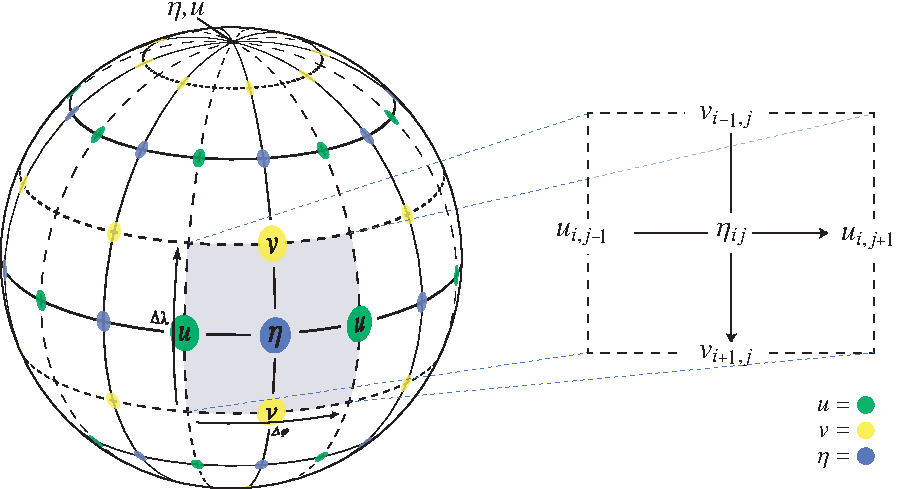
\includegraphics[width=0.8\linewidth]{Figures/GridDiagram_revision}
\caption{The staggered grid structure used in ODIS. A single cell is show on the right of the figure, where surface displacement, $\eta$, represents a cell centered quantity. $u$ velocity nodes are staggered eastward of $\eta$, whereas $v$ velocity nodes are staggered southwards. Both $u$ and $v$ are defined at the cell walls. Lines of meridian merge to singularities at the poles, where a single $\eta$ and multiple $u$ nodes are stored.\label{fig:grid}}
\end{figure}

\subsection{Tidal Quality Factor}

A useful parameter for understanding tidal dissipation is the quality factor, $Q$. Defined as the ratio of maximum energy stored to the total energy dissipated in a purely elastic body, small values of $Q$ correspond to a dissipative environment \citep{goldreich1966q}. \citet{tyler2011tidal} and \citet{matsuyama2014tidal}, however, use the kinetic energy $E_k$ of the fluid system to represent the energy stored in the tide;

\begin{equation}\label{eq:Q}
Q \equiv 2 \pi \dfrac{\text{max} \left( E_{k} \right)}{E_{diss}} = \dfrac{\Omega}{2 \alpha}
\end{equation}

where the total time averaged dissipation is $E_{diss}$. This definition is ill-defined, however, as the the kinetic and dissipated energy in the ocean tide are intrinsically coupled. Large drag coefficients enhance dissipation, but this demands a decrease in the kinetic energy of the system, which in turn results in a reduction in velocities and consequently dissipation. This coupling makes it difficult to use a definition of $Q$ that is meaningful to the Planetary Science community. We suggest that a more appropriate definition would be using the maximum stored energy in the equilibrium tide (i.e., the theoretical instantaneous tide raised in the absence of dissipation) in the numerator of Equation \ref{eq:Q}, which is used in dissipation studies of gas planets \citep{goldreich1966q}. For the remainder of this work, however, we return to simply presenting our results as a function of drag coefficient, rather than potentially misleading readers with alternate definitions of $Q$. 

\subsection{Numerical Model \label{subsec:model}}

In this section we outline our two dimensional, finite difference computational fluid dynamics (CFD) model, known as Ocean Dissipation in Icy Satellites (ODIS). In its current form, ODIS is based extensively on the models discussed in and developed by \citet{zahel1973diurnalk,zahel1978influence} and \citet{sears1994tidal,sears1995tidal}. We first provide a description of the numerical grid. An overview of the finite difference scheme itself is then given, before summarising and illustrating limitations of the finite difference scheme and grid choice.

\subsubsection{Discretized Grid \label{subsec:grid}}

We employ a fixed latitude-longitude grid for our numerical simulations, defined in a spherical coordinate system. The grid is constructed in a staggered manner, meaning that velocity nodes are placed to the east and south of their parent displacement nodes. \textbf{This is identical to the Arakawa ``C'' grid introduced by \citet{arakawa1977computational}}. This is illustrated in Figure \ref{fig:grid}, where we define $u$ and $v$ as the eastward and northward velocity components, respectively. $\Delta \lambda$ is the grid spacing in latitude, whereas $\Delta \phi$ is the grid spacing in longitude. A staggered approach is adopted as it avoids numerical oscillations that grow in the solution by calculating derivatives \textit{between} grid nodes rather than over them. This is discussed further in section \ref{subsec:fd_expan}.

As is clear from Figure \ref{fig:grid}, lines of meridian all converge to single points at either pole. Consequently, the model is forced to go from $m$ longitudinal grid points immediately surrounding the pole to merely a single point at the pole itself. Accordingly, single values of $\eta$ are stored at each pole, whereas multiple $u$ values are required to maintain numerical stability. 

ODIS stores three separate 2D arrays for $\eta$, $u$ and $v$. They are accessed in a parent-child configuration, whereby the velocity nodes immediately east and south of a displacement node are the children to their parent $\eta$. Both $u$ and $v$ at the southern and eastern walls of the cell in Figure \ref{fig:grid} are children to the central $\eta$ node. % This is of little importance to the model's computations, but does lend some insight into the infrastructure of ODIS.

\subsubsection{Finite Difference Expansions \label{subsec:fd_expan}}

In order to solve the LTEs, we expand equations \ref{eq:mass_lin} and \ref{eq:mom_lin} in a semi-implicit finite difference scheme in spherical coordinates \citep{sears1995tidal}. \textbf{Details of the coordinate transform for these equations are given in \ref{app:coords}.} Expanding $\bm{u}$ into its components and assuming $\eta \ll h_0$, the momentum equation becomes,

\vspace{-0.6cm}
\begin{equation}
u_{ij}^{t+1} \approx  \left[ \,2 \Omega \bar{v}_{ij}^{\textbf{t}} \sin{\lambda_i} \vphantom{\frac{c_D}{h_0}\sqrt{\left(u_{ij}^{t}\right)^2}} - \alpha u_{ij}^{t} \right. \\ 
- \frac{c_D}{h_0}\sqrt{\left(u_{ij}^{t}\right)^2 + \left(\bar{v}_{ij}^{t}\right)^2}\cdot u_{ij}^{t} - \frac{g}{R \cos{\lambda_i}} \frac{\partial \eta_{ij}^{t}}{\partial \phi_j} \\  
+ \left.\left(1 + k_2 - h_2\right) \frac{1}{R \cos{\lambda_i}} \frac{\partial U_{2,ij}^{t}}{\partial \phi_j} \right]  \Delta t + u_{ij}^{t} \, , \label{eq:momu_fd}
\end{equation}
\vspace{-0.6cm}
\begin{equation}
v_{ij}^{t+1} \approx  \left[ \,-2 \Omega \bar{u}_{ij}^{\textbf{t}} \sin{\lambda_i} \vphantom{\frac{c_D}{h}\sqrt{\left(u_{ij}^{t}\right)^2}} - \alpha v_{ij}^{t} \right. \\ 
- \frac{c_D}{h_0}\sqrt{\left(\bar{u}_{ij}^{t}\right)^2 + \left(v_{ij}^{t}\right)^2}\cdot v_{ij}^{t} - \frac{g}{R} \frac{\partial \eta_{ij}^{t}}{\partial \lambda_i} \\  
+ \left.\left(1 + k_2 - h_2\right) \frac{1}{R} \frac{\partial U_{2,ij}^{t}}{\partial \lambda_i} \right]  \Delta t + v_{ij}^{t} \, , \label{eq:momv_fd}
\end{equation}

\noindent and the continuity equation becomes, 

\begin{equation}
\eta_{ij}^{t+1} \approx 
-\frac{h_0}{R \cos{\lambda_i}}\left[
\frac{\partial \left(v_{ij}^{t+1} \cos{\lambda_i}\right)}{\partial	\lambda_i}  
+\frac{\partial u_{ij}^{t+1}}{\partial	\phi_j}\right]
\Delta t
+ \eta_{ij}^{t}\, . \label{eq:mass_fd}
\end{equation}

Latitude and longitude are denoted by $\lambda$ and $\phi$ respectively. $i$ and $j$ represent the $i\text{th}$ and $j\text{th}$ latitude and longitude nodes within the grid. The time index is given by $t$, and $\Delta t$ represents the time-step. Overbars correspond to spatial averages, a necessity given the staggered nature of the grid. Spatial and temporal expansions are made using the Euler method and are first order accurate in space and time.

All derivatives of the degree-2 tidal potential (equations \ref{eq:U_ecc} and \ref{eq:U_obliq}) have analytical solutions, and thus do not require further finite difference expansion. Derivatives of all other quantities, however, do require further expansion. The expansions take the general form of either,

\begin{align}
\frac{\partial w_{ij}^{\textbf{t}}}{\partial \lambda} &\approx \frac{w_{i+\nicefrac{1}{2},j}^{\textbf{t}} - w_{i-\nicefrac{1}{2},j}^{\textbf{t}}}{\Delta \lambda} \, , \label{eq:gen1}
\end{align} or,

\begin{align}
\frac{\partial w_{ij}^{\textbf{t}}}{\partial \phi} &\approx \frac{w_{i,j+\nicefrac{1}{2}}^{\textbf{t}} - w_{i,j-\nicefrac{1}{2}}^{\textbf{t}}}{\Delta \phi} \, , \label{eq:gen2}
\end{align}

\noindent where $w$ represents $u$, $v$ or $\eta$.

Equations \ref{eq:gen1} and \ref{eq:gen2} show that each derivative is evaluated halfway between the nodes where $w$ is stored. Consequently, any derivative of $w$ is calculated at a position held by a different variable because the grid is staggered. For example, $\partial_\phi u_{ij}$ is always evaluated at the position held by $\eta_{ij}$ as $u_{i,j-\nicefrac{1}{2}}$ and $u_{i,j+\nicefrac{1}{2}}$ lie to the left and right of $\eta_{ij}$,  respectively. This is shown clearly on the right of Figure \ref{fig:grid}.

\subsubsection{Numerical Scheme}

ODIS begins its calculations by (1) determining the mass of each volume element in the initial ocean assuming an undisturbed ocean of thickness $h_0$. With the mass calculated in each cell, it is then possible to find the dissipated energy in the system.

The next step in the numerical integration is to calculate $\nabla U_2$ across all $u$ and $v$ grid points (2). This gives the initial force per unit mass experienced by a fluid element in the model domain.

Once the tidal acceleration is known, ODIS directly calculates $u$ and $v$ over the grid by solving equations \ref{eq:momu_fd} and \ref{eq:momv_fd} (3). This step is purely explicit as $u$ and $v$ depend only on information from the previous time step, $t$. Following this, $\eta$ is then updated using the new velocity values (4). In contrast to the velocity calculations, this step is semi-implicit as it relies on values from both the current and previous time steps, as shown in Equation \ref{eq:mass_fd} \citep{sears1995tidal}.

After solutions for $u$, $v$, and $\eta$ are found at the new time step, $t+1$, the energy calculations begin (5). For Rayleigh drag, ODIS calculates and stores global dissipated energy flux as,

\begin{equation}
F_{\alpha}^{t+1} = \frac{1}{4 \pi R^2 }\sum_{i=1}^{n} \sum_{j=1}^{m} \alpha \textbf{M}_{ij} \left[\left(u_{ij}^{t+1}\right)^2 + \left(v_{ij}^{t+1}\right)^2\right] \, , \label{eq:E_alpha}
\end{equation}

for $n$ and $m$ grid points in latitude and longitude, respectively. The summed terms in Equation \ref{eq:E_alpha} give the total dissipated energy in the system across the current time step, \textbf{for the total ocean column mass $\textbf{M}$ within each cell}. The factor in front of the summations then averages this quantity over the satellite's surface area giving $F_{\alpha}$ in watts per square metre. For bottom drag the equivalent expression is

\begin{equation}
F_{c_D}^{t+1} = \frac{1}{4 \pi h_0 R^2 }\sum_{i=1}^{n} \sum_{j=1}^{m} c_D M_{ij} \left[\left(u_{ij}^{t+1}\right)^2 + \left(v_{ij}^{t+1}\right)^2\right]^{\nicefrac{3}{2}}\, . \label{eq:E_cd}
\end{equation}

Every time step calculations 2-5 are repeated, beginning with determining $\nabla U_2$. Finally, at the end of each orbit, $F_\alpha$ or $F_{c_D}$ is summed and averaged over the orbital period (6). This gives the time and surface averaged heat flux due to tidal dissipation for Rayleigh drag,

\begin{align}
\left\langle F_\alpha \right\rangle_{orbit} &= \frac{1}{p}\sum_{t=1}^{p} F_{\alpha}^{t}  \, , \label{eq:E_alpha_orbit}
\end{align} 
and bottom drag,

\begin{align}
\left\langle F_{c_D} \right\rangle_{orbit} &= \frac{1}{p}\sum_{t=1}^{p} F_{c_D}^{t}  \, , \label{eq:E_cd_orbit}
\end{align}

where $p = \nicefrac{T}{\Delta t}$, the total number of time steps in the orbital period, $T$. These expressions are consistent with \citet{sears1995tidal}.

Steps 2-6 are repeated until the model has converged into a periodic equilibrium. Care must be taken when selecting convergence criteria. Simulations involving thick oceans and small drag coefficients will oscillate about their converged solution with periods of \numrange{10}{100} orbits or more due to the large inertia associated with thick, poorly dissipative oceans (see Figure \ref{fig:conv_a}). These simulations clearly require longer run-time. For the most time consuming simulations, we take the mean dissipation over one full oscillatory cycle.

\begin{figure}
\centering
\includegraphics[width=0.85\linewidth]{Figures/spatial_error_ecc}
\caption{\textbf{Displacement solutions (left column) and corresponding percentage error (right column) for Enceladus' eccentricity tide with $h_0 = \SI{500}{\metre}$ and $\alpha = \SI{e-5}{\per\second}$. The numerical grid was spaced at \SI{1}{\degree}. Each row corresponds to a different time interval throughout one orbital period, $T$. Percentage eror is  $< \SI{0.01}{\percent}$ over much of the model domain, with local highs where the solution passes from postive to negative displacement.} \label{fig:spatial_error}}
\end{figure}


\subsubsection{\textbf{Numerical Tests} \label{subsubsec:num_test}}

As with any numerical solution there are errors associated with discretisation of the problem into the model domain. We performed resolution testing across various ocean thicknesses to determine how these errors scale with grid resolution \textbf{using the semi-analytical solutions of \citet{matsuyama2014tidal} as our benchmark in all following numerical tests. Although the solutions from \citet{matsuyama2014tidal} are not purely analytical, we use solutions that are truncated at spherical harmonic degree $l=20$. As such, these can be considered the exact solutions. Four of these tests are shown in this section to illustrate that the numerical method and code perform as expected, both as a function of space and time. Each test shown here was run for Enceladus' eccentricity tide, using $h_0 = \SI{500}{\metre}$, $\alpha = \SI{e-5}{\per\second}$, and $\Delta t = \SI{2}{\second}$. The grid was spaced at \SI{1}{\degree} throughout, except in tests 3 and 4 which examine how the numerical error depends on model resolution.}

\begin{figure}[t]
\centering
\includegraphics[width=\linewidth]{Figures/temporal_error_ecc}
\caption{\textbf{Normalised error norms as a function of time for Enceladus' eccentricity tide with $h_0 = \SI{500}{\metre}$ and $\alpha = \SI{e-5}{\per\second}$. At approximately \num{10} orbits, all parts of the solution have converged after which the normalised error remains small, and oscillates over the orbital period.} \label{fig:temporal_error}}
\end{figure}


\begin{figure}[t]
\centering
\includegraphics[width=0.6\linewidth]{Figures/convergence_eta}
\caption{\textbf{Normalised error norms as a function of time for Enceladus' eccentricity tide with $h_0 = \SI{500}{\metre}$ and $\alpha = \SI{e-5}{\per\second}$, taken at pericenter at the beginning of orbit \num{100}. A least-squares fit to each error norm in log-log space yields slopes of \num{0.86}, \num{0.90} and \num{1.03} for the $L_1$, $L_2$ and $L_{\infty}$ normalised error norms, respectively.} \label{fig:spatial_convergence}}
\end{figure}



\begin{figure*}[!t]
    \centering
    \begin{subfigure}[t]{\linewidth} % contains the two plots in a single figure
        \includegraphics[width=\linewidth]{Figures/convergence2}
        \phantomcaption
        \label{fig:conv_a}
    \end{subfigure}
    \begin{subfigure}[t]{0\linewidth} % the hidden unwanted image
         \includegraphics[width=\linewidth]{Figures/convergence2}
         \phantomcaption
         \label{fig:conv_b}   
    \end{subfigure}
    \vspace{-0.5cm}
\caption{Dissipation convergence and error scaling as a function of grid resolution. Panel \ref{fig:conv_a} shows the time evolution of the orbit-averaged dissipated energy at periapsis. The solid lines represents different grid resolutions, whereas the dashed line is the semi-analytical solution for Rayleigh drag from \citet{matsuyama2014tidal}. Panel \ref{fig:conv_b} shows the \textbf{dissipation} error between the numerical and semi-analytical solutions with increasing resolution. The least-squares slope of the first six data points (when the slope is steady) in log-log space is \num{1.94}. These simulations are for the obliquity tide using $h_0 = \SI{1}{\kilo\metre}$ and $\alpha = \SI{e-8}{\per\second}$ on Titan. \label{fig:conv}}
\end{figure*}

\textbf{It is important to understand how the model resolves the solution across the numerical domain, especially when using the fixed latitude-longitude grid employed here. This is done in test 1 (Figure \ref{fig:spatial_error}) where the ocean surface displacement (left) is compared to the corresponding error field (right). The ocean configuration is near a gravity-wave resonance, so it is easy to discern the eastward propagating gravity-wave through the model domain at each time slice. Note that at pericentre ($t/T = 0$) positive displacements are at a maximum, while at apocentre ($t/T = 0.5$) they are at a minimum. The percentage error in the numerical model is very small ($< \SI{0.01}{\percent}$) over the majority of the domain. Near the poles, where grid points are closely arranged, numerical error is smallest. At the zero-crossing in displacement both the numerical and semi-analytical solutions become $\ll \SI{1}{\metre}$. As a result, the numerical error locally spikes in those regions producing the rings of high error seen in Figure \ref{fig:spatial_error}. Overall, the numerical error is very low, giving us confidence in the ability of ODIS to spatially resolve the solutions.}  

\textbf{As the tidal forcing in this problem is periodic, one expects the solution and its corresponding error to also be periodic. It is therefore logical to investigate how the numerical error changes over time. We investigate this in our second test, starting the numerical simulations from an undisturbed and unforced ocean. This is shown in Figure \ref{fig:temporal_error}, where once again the numerical error is computed against the \citet{matsuyama2014tidal} semi-analytical solutions. The error is quantified using the normalised $L_1$, $L_2$ and $L_{\infty}$ error norms (defined in \ref{app:error}). The maximum error in each solution if given by the $L_{\infty}$ norm. Normalised error is greatest at the beginning of the simulation, as this is during the model ``spin-up'' time. After approximately \num{10} orbits both the displacement and two velocity solutions converge. At this point the average error over each orbital period remains constant. The magnitude of this converged error is a function of the grid resolution, as shown in test 3. Once converged, the normalised error oscillates over the orbital period. This is expected, as the maximum gradients in all three solutions periodically vary an orbit. In regions where these gradients are maximised the finite difference scheme produces the poorest approximation. Consequently, the error varies as a function of time, even after convergence.  Although not shown, the simulation remains stable for over 1 year of simulation time. }

\textbf{In order to verify if the numerical scheme is implemented properly, it is prudent to perform convergence analysis on the numerical solution. Figure \ref{fig:spatial_convergence} shows this analysis in our third test. The normalised error norms are plotted with varying grid resolution, spanning \SIrange{1}{10}{\degree} in both longitude and latitude. As expected, the accuracy of the numerical solution increases with decreasing grid size. With increasing resolution the local approximation of spatial derivatives improves, which is what produces this general trend. The rate at which the errors are reduced as a function of resolution is known as the order of convergence. This can be estimated by finding the slope of the normalised error norms in log-log space. Using a least-squares fit we find slopes of \num{0.86}, \num{0.90} and \num{1.03} for the $L_1$, $L_2$ and $L_{\infty}$ normalised error norms, respectively. We therefore conclude that the order of convergence of the numerical method implement in ODIS is $\sim 1$, which is expected for the finite difference expansions made in equations \ref{eq:gen1} and \ref{eq:gen2}.}

\textbf{The total dissipated energy is of fundamental importance from the view of the Planetary Science community. As our final test we therefore investigate how the numerical dissipation solution varies as a function of time and grid resolution, shown in Figure \ref{fig:conv}. Unlike the other tests, this is run for the obliquity tide on Titan with an ocean of $h_0 = \SI{1}{\kilo\metre}$ and $\alpha = \SI{e-8}{\per\second}$. The numerical time- and obrbit-averaged dissipated energy oscillates over time until converging to a single value, shown in the left panel. This final value gradually approaches the \citet{matsuyama2014tidal} semi-analytical solution as grid resolution is increased. The right panel, similar to Figure \ref{fig:spatial_convergence}, plots the numerical percentage error as a function of grid space. Again, the error decreases with decreasing grid space. The order of convergence for the dissipation is once again given by the slope of the line in Figure \ref{fig:conv_b}, which approaches $\sim 2$. As dissipated energy scales with the square of the velocity field, second order convergence is expected. Note that this does not mean the implemented numerical scheme is second order accurate. } 

Based on these resolution tests, all further simulations were ran for grid resolutions of \SIrange{1}{3}{\degree} in latitude and longitude.

\subsubsection{\textbf{Timestep and Grid Limitations} \label{subsubsec:grid_limits}}

A natural issue arising from the choice of grid is the time step used. As described in section \ref{subsec:grid}, the fixed latitude-longitude grid causes meridian lines to converge at the poles. Nodes near each pole therefore have much smaller spatial separations than those at the equator. In order to satisfy the Courant-Friedrichs-Lewy (CFL) condition required for numerical stability, we are forced to select sufficiently small time-steps based on the minimum node spacing and characteristic ocean flow time-scale \citep{arakawa1977computational,sears1995tidal}. \textbf{The maximum speed information can travel around the model domain is at the shallow water gravitational wave speed, $\sqrt{gh_0}$ \citep{lamb1932hydrodynamics}. Correspondingly, the CFL constraint on the time step is $\Delta t \leqslant \Delta x / \sqrt{gh_0}$, where $\Delta x$ is the minimum grid spacing in the model domain. Note that the maximum time step for numerical stability is a function of the ocean thickness as well as grid resolution. As $\Delta x$ is smallest surrounding the poles, this forces a severe constraint on the time step. This constraint is often referred} to as the ``pole problem''. \textbf{For a \SI{1}{\degree} resolution grid with a \SI{10}{\kilo\metre} thick ocean on Titan and Enceladus, the maximum possible time step is \SI{6.7}{\second} and \SI{2.3}{\second}, respectively.} Several workarounds to ease the time step have been applied throughout the literature \citep{comblen2009finite}. For example, it is common to apply a Fourier filter to remove high wavenumber components of the solution near the poles \citep{murray2002fourier}, or to use the spectral transform method as reviewed by \citet{swarztrauber1996spectral}. In this work, however, we apply none of these methods, and obey the CFL condition by selecting the appropriate time step for the model resolution.

\begin{figure}[!b]
\centering
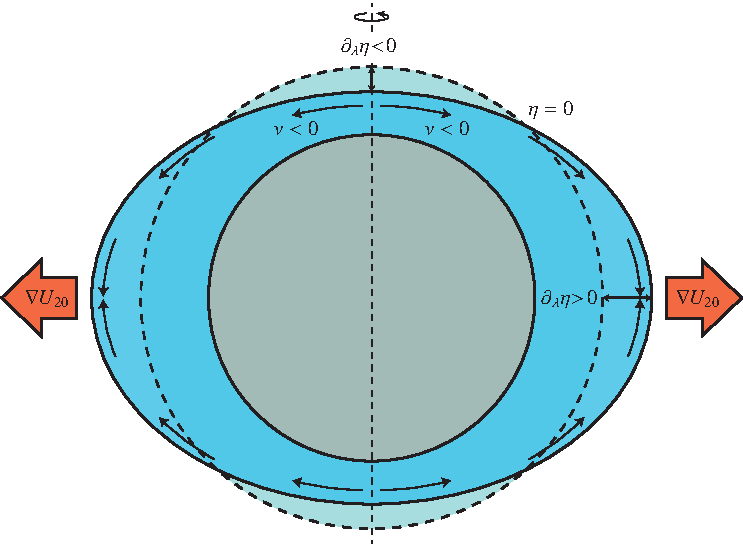
\includegraphics[width=0.7\linewidth]{Figures/CoordProb}
\caption{Schematic representation of the ocean tide due to the eccentricity-radial tidal potential ($U_{20}$), at periapsis. Taking the derivative of $v$ across the north pole yields a zero result in the spherical coordinate system, despite the clear mass divergence away from the poles which should result in $\partial_{\lambda} \eta < 0$.\label{fig:coord_prob}}
\end{figure}

A more significant issue arises from the combined choice of coordinate system and grid structure. Nodes located directly at the poles become singularities in space, as the normal directions east and west used to define the velocity components become meaningless. Consider the northward velocity flow near the north pole under the eccentricity-radial tide, shown in Figure \ref{fig:coord_prob}. Conservation of mass and the formation of an equatorial bulge force flow to diverge away from the pole. In solving for the surface displacement node directly at $\lambda = 90^{\circ}$, we must take the derivative of $v$ across the pole (as in Equation \ref{eq:momv_fd}). As each $v$ node located either side of the pole has the same magnitude and, perhaps unintuitively, is orientated in the same direction (southwards), this derivative becomes zero.  This forces surface displacement at the pole to zero as well. Yet, as there is divergence away from the pole, it is required that $\partial_{\lambda} \eta < 0$ to conserve mass. Clearly, the choice of coordinate system and grid do not permit such behaviour at the poles. 

To work around this problem, we employ both first-order accurate one dimensional Euler interpolation and third-order accurate Lagrange interpolation for all $u$ and $\eta$ nodes located at the pole, avoiding the need to directly solve for these points. We then take the mean of the interpolated $\eta$ points and prescribe that as the polar value. For $u$, the mean is taken for the eccentricity tide as eastward velocity tends towards zero at the poles. Average velocity is not computed for the obliquity tide, however, as non-zero eastward velocity components exist at the poles.

\subsection{Model Runs and Parameters \label{subsec:param}}

\begin{table}[!t]
\scriptsize
\centering
\begin{tabularx}{\linewidth}{p{1.5cm} p{2.5cm} p{2.5cm}}
 \toprule
Parameter & Description & Value\\
 \midrule \midrule
$\Omega$ & angular velocity & $4.55 \times 10^{-6} \, \si{\radian\per\second}$\\
$r$ & satellite radius & $2574.7 \, \si{\kilo\metre}$\\
$a$ & semi-major axis & $1.221865 \times 10^6 \, \si{\kilo\metre}$\\
$g$ & surface gravity & $1.35 \, \si{\metre\per\second\squared}$\\
$e$ & eccentricity & $0.0288$\\
$\theta_0$ & obliquity & $0.32^{\circ}$\\
$k_2$ & tidal Love number & $0.120$\\
$h_2$ & tidal Love number & $0.2$\\
 \bottomrule
\end{tabularx}
\caption{Model parameters used in all simulations presented here. All values are specific to Titan, and are taken from \citet{zebker2009size,chen2013tidal}.  \label{tb:param}}
\end{table}

We first perform both semi-analytical and numerical simulations for Titan and Enceladus under the eccentricity and obliquity tides. For each tidal component over 3000 simulations were run for \hbox{$h_0 = 1 - 10^4 \, \si{\metre}$} and \hbox{$\alpha = 10^{-9} - 10^{-5} \, \si{\per\second}$}. Such resolution is necessary to capture resonant features. The semi-analytical solution for the time averaged surface heat flux from \citet{matsuyama2014tidal} was directly compared to the numerical values to reveal any inaccuracies in the numerical solution across this parameter space. 

Following testing and verification of the numerical solutions for Rayleigh drag, ODIS was then run using only bottom drag for \hbox{$h_0 = 1 - 10^4 \, \si{\metre}$} and \hbox{$c_D = 10^{-7} - 10^{-1}$}. These simulations were again run for both the eccentricity and obliquity tides. With results for both Rayleigh and bottom drag we were able to compare tidal dissipation between these two drag regimes. The model parameters used for both Titan and Enceladus are shown in Table \ref{tb:param}.

Numerically solving the LTEs to convergence is a computationally expensive process. As shown in Figure \ref{fig:conv_a}, convergence will only be reached after a significant amount of simulation time. The example given in Figure \ref{fig:conv_a} was run using initial conditions for a stationary, undisturbed ocean. To speed up convergence we employ the technique used by \citet{sears1995tidal}, whereby the final output of one simulation is used as the initial condition for the next simulation. Upon completion, each simulation will spawn one to two `child' simulations. These new simulations will in turn spawn their own `children' once they are complete. This method of solving over such a large parameter space helps to significantly reduce computational run and spin-up time. Several tests were also run to ensure that a given simulation would converge to a single solution, regardless of initial condition.



